\documentclass[]{report}   % list options between brackets
\usepackage{titlesec}
\usepackage{hyperref}
\usepackage[margin=1.25in, footskip = 0.5in]{geometry}
\usepackage{graphicx}
\usepackage{subcaption}
\usepackage{placeins}
\usepackage{appendix}

\titleformat{\chapter}[display]
{\normalfont\huge\bfseries}{}{20pt}{\Huge}   
\titlespacing*{\chapter}{0pt}{-50pt}{40pt}

\titleformat{\title}
	{\Large\bfseries}{}{0pt}{\huge}

% type user-defined commands here

\begin{document}

\title{Something about Submitter Segmentation}   % type title between braces
\author{Anna Marbut}         % type author(s) between braces
\date{May 2019}    % type date between braces
\maketitle


\chapter*{Executive Summary}
\label{execsum}
\addcontentsline{toc}{chapter}{\nameref{execsum}}
  This is where the executive summary goes



\tableofcontents

\chapter{Introduction}

Submittable was founded in 2010 by three software developers who were creatives when they were off the clock -- one novelist, one musician, and one filmmaker. All three had experience with the submission process for creative work, and saw a need for improvement. This process varied for every opportunity: one organization might want to be mailed a physical copy of the work, another might want to be mailed a thumb drive, another might receive submissions via e-mail, and yet another might use a digital filesharing service. Submittable's founders had experience with the frustrating variety of requirements on one side, but they quickly realized how much worse it was for the organizations receiving the submissions. These organizations were using physical filing systems, spreadsheets, e-mail chains, and any other number of quasi-structured methods to track the submissions that they'd received and the various communications, review processes, and administrative tasks related to them. This left a lot of room for human error and increased frustration on both sides of the whole process.

With these issues in mind, Submittable's founders set out to create a platform which could accept all of the most common filetypes (even very large files) and streamline the entire submission management pipeline. Almost 10 years later, Submittable has helped 15 thousand organizations collect and manage over 12 million submissions. While the bulk of their clients remain in the creative realm (literary journals, film contests, photography journals, auditions, etc.), they have branched out into almost every industry in which any type of submission needs to be made (research grants, job applications, charitable foundations, residency programs, etc.), and the number of these other clients is growing quickly. The company has grown from three founders to 70 employees, was picked up by the startup incubator Y-Combinator (known for DropBox, AirBnB, Weebly, and others), and has received over \$5 million in venture capital funding. In short, the founders' idea seems to have been a good one.

Submittable's business model has been one of ``software-as-a-service", or SAAS, in which their clients pay a subscription fee for use of the software platform. Different subscription levels are available based on which features each organization wants to use. Available features include the number of active opportunities allowed (also referred to as ``calls to submission" or ``forms"), the option for multiple reviewers, gallery voting (such as for public photography contests), submission fee collection, and automated reporting. As the business has grown, the list of features offered to client organizations has expanded from those immediately related to software functionality, to more abstract features such as hosting an opportunity on a custom url, white-labelling the software, or providing marketing services to promote a specific opportunity or organization. This last feature is the inspiration and focus for this project.

When a client opts for a subscription package that includes marketing services, they work with Submittable's marketing team to design a custom campaign for the client's opportunity/opportunities. This campaign can include anything from social media outreach, blog posts, newsletter articles, and custom reminders to interested submitters. Almost always, a marketing campaign also includes an e-mail campaign to a targeted list of Submittable's users (aka submitters). Currently, these lists are populated by matching users (who have opted to be on the marketing services list) based on the use of campaign-specific keywords in their personal description, submission cover letter, or in the description or name of opportunities to which they've submitted. While this method makes a pretty good guess at which submitters would be interested in the campaign, it is a broad way to segment the submitter base, and is likely to both include some submitters who won't be interested and leave out some who would be. 

In this project, we will explore using an adaptation of the PageRank algorithm to rank submitters based on their interest in a specific topic. The goal is to provide Submittable with a more robust method for selecting which submitters should be contacted for a specific marketing campaign. Improving the quality of these lists will improve the experience for both the client and the submitter, with clients reaching users and receiving submissions that are a better fit for their opportunities, and submitters receiving promotions about opportunities to which they are more likely to submit. 

AND THEN WRAP IT UP SOMEHOW

\chapter{Background}
\section{Classification algorithms}

--- supervised vs. unsupervised

--- ADA clustering?

--- machine learning

--- SVM and other supervised techniques?

\textbf{twitter user profling: https://www.aaai.org/ocs/index.php/ICWSM/ICWSM11/paper/viewFile/2886/3262}

--- gradient boosted decision trees

\textbf{classifier comparisons: https://ieeexplore.ieee.org/abstract/document/5170933}

--- Naive bayesian, Instance-based learner, classification and regression tree, Naive Bayesian tree

\textbf{twitter user classification: https://dl.acm.org/citation.cfm?id=1871993}

--- stacked-SVM

\section{Google PageRank}

\textbf{twitter community identification: http://snap.stanford.edu/networks2013/papers/netnips2013\_submission\_3.pdf}

--- used pagerank to identify central communities and community members in twitter network

\textbf{Multilabel user classification using the community structure of online networks: https://journals.plos.org/plosone/article?id=10.1371/journal.pone.0173347}

--- inferring user interests based on sparsely annotated user profiles

--- use pagerank to identify most important community memberships for each user, then apply to graph embeddings

\textbf{Personalized PageRank Estimation and Search: https://arxiv.org/abs/1507.05999}

--- bidirectional personalized pagerank; meant to increase speed of search, but may be useful in bidirectional network (ie. submitters w/ common opportunities)

\textbf{Identifying Key Users in Online Social Networks: https://epub.uni-regensburg.de/25914/1/Identifying\_Key\_Users\_in\_Online\_Social\_Networks\_1.pdf}

--- importance of connectivity in marketing basedd on social networks

--- concept of eigenvector centrality to acknowledge inequality of importance in network nodes

--- uses weighted vector to apply bias for high-low activity users; \textbf{ bidirectional activity weights; address undirected connectivity}

--- used dampening = 0.85; supported that higher d does not drastically change order of high ranking results, but takes much longer

\textbf{Edge-Weighted Personalized PageRank: http://wenleix.github.io/paper/edgeppr.pdf}

--- node vs. edge weights; ie importance of submitter vs importance of relationship between submitters; in our context, node weight could be seen as topicality of submitter (how many labeled opportunities submitted to, keywords in user description), edge weight could be seen as topicality of opportunity that submitters have in common (\# of relevent labels, keywords in opportunity description)

--- focuses on providing quick(er) solution for applying edge weights to pagerank

--- use reduced model of edge-weighted pagerank to decrease computation time

\textbf{Topic-Sensitive PageRank:http://www-cs-students.stanford.edu/~taherh/papers/topic-sensitive-pagerank.pdf}

--- use pre-computed topic-specific pagerank vectors to rank search results; avoids highly connected nodes from rising to top when not topical

--- pagerank matrix must be irreducible (highly connected, limited clustering?) and aperiodic (no sinks, solved by damping factor)

--- topic bias added @ damping factor: $\alpha \vec{p}$ where $\alpha = P(teleportation)$ and $\vec{p} = 1/N$ or $\vec{p} =$ biased rank vector

--- power iteration looks like: $\vec{Rank} = (1- \alpha )M * \vec{Rank} + \alpha \vec{p}$; so that biased rank is added at each iteration? how does it ever reach convergence? Wouldn't there always be difference of damping factor?

--- reiterates that value of $\alpha$ does not have significant effect on ordering of results; this study used $\alpha = 0.25$

\textbf{TwitterRank: https://ink.library.smu.edu.sg/cgi/viewcontent.cgi?article=1503\&context=sis\_research}

--- topic-senstive ranking of influential tweeters

--- defines social network homophily: social networks are homogeneous with regard to manny sociodemographic, behavioral, and inntrapersonal characteristics; ie. "friends" follow each other b/c they have similar interests

--- use LDA to give topic-scores for each tweeter based on aggregate of tweet text

--- use topic scores to weight transition matrix; not just straight probability of random surfing, but weighted for topic similarity; damping factor is also topic-specific, another result of LDA

--- nice ideas for visualizing connectivity

--- topics poorly described, not cohesive since only based on unsupervised classification


\chapter{Data and Descriptive Statistics}         
\section{Data Source}
The data for this project comes from an Amazon Redshift Database that Submittable has set up to perform basic analytic queries about their clients, users, and product usage. Due to the scope of this research, the data used is centralized around Submittable's users, including information that they've explicitly provided on their Submittable profile, as well as information about the various submissions that they've made. In accordance with Submittable's privacy policy, no information that could be used to identify an individual user was included in the data for this project.

\section{User Accounts}
Submittable has 4.2 million users from all time, 770K of whom made a submission in 2018. As seen in Figure \ref{fig:userCreate}, the number of new user accounts has increased exponentially, with almost twice as many new accounts in 2018 as there were in 2017. The number of users making at least one submission is also increasing steadily each year, although on a linear scale with about 100K more active submitters each year since 2013 (Figure \ref{fig:userSubmit}). On average Submittable users have made five submissions in their account lifetimes, with the number of submissions that an individual user has made ranging from one to 7.4K. Additionally, 62\% of submittable users have only made one submission since they created their account.
\begin{figure}[h]
    \centering
    \begin{minipage}{0.45\textwidth}
        \centering
        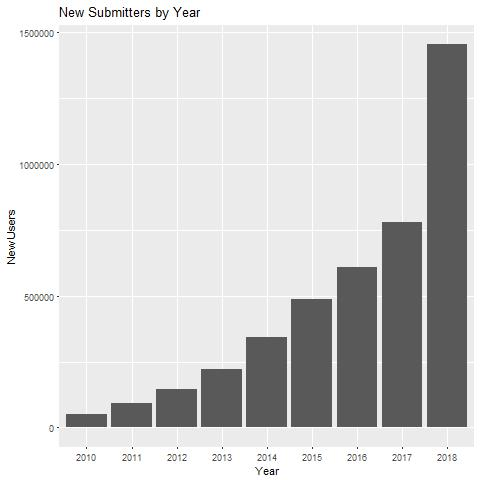
\includegraphics[width=1\textwidth]{userCreate_plot.jpg} % first figure itself
        \caption{New Submittable User Accounts by Year}
	  \label{fig:userCreate}
    \end{minipage}\hfill
    \begin{minipage}{0.45\textwidth}
        \centering
        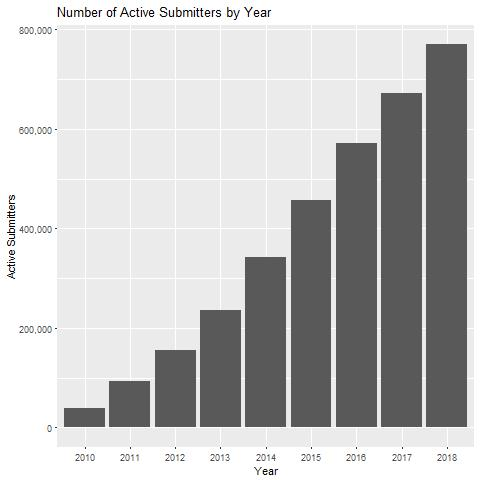
\includegraphics[width=1\textwidth]{userSubmit_plot.jpg} % second figure itself
        \caption{Submittable Users with at least One Submission by Year}
	  \label{fig:userSubmit}
    \end{minipage}
\end{figure}
\FloatBarrier
In creating a Submittable account, each submitter has the option to provide a written description of themselves and various demographic information. Roughly 100K submitters have something written in their description field, and a brief scan shows that these are fairly descriptive, like what would be included in a cover letter or a professional biography. 1.2 million of Submittable's users have provided location information, hailing from 244 countries and territories. However, 75\% of these users are from the United States, and 91\% of them are from the top ten countries shown in Table\ref{table:userCountry}. 

\begin{figure}[h]
\centering
\begin{minipage}{0.45\textwidth}
     \centering
\captionof{table}{Top Ten Submittable Users' Countries}
\label{table:userCountry}
\begin{tabular}{rlr}
  \hline
 & Country & Number of Submitters \\ 
  \hline
1 & United States & 913542 \\ 
  2 & United Kingdom & 59268 \\ 
  3 & Canada & 56316 \\ 
  4 & Australia & 26898 \\ 
  5 & India & 22709 \\ 
  6 & Nigeria & 7458 \\ 
  7 & Germany & 7359 \\ 
  8 & France & 5652 \\ 
  9 & South Africa & 5578 \\ 
  10 & Italy & 5451 \\ 
   \hline
\end{tabular}
    \end{minipage}
\end{figure}
\FloatBarrier

\section{Opportunities and Submissions}
Submittable's software platform has hosted a total of ~130K opportunities, with a fairly steady increase of 3-5K new opportunities created every year except for 2018 (Figure \ref{fig:formYear}). This decrease in new opportunities last year can likely be attributed to the maturation of many client accounts, who are now re-using forms that they've created in previous years. This is also supported by the steady increase in the total number of submissions made each year, including last year, which has increased by ~300K every year since 2010 (Figure \ref{fig:subYear}). In its lifetime, Submittable has received a total of 12M submissions.

\begin{figure}[h]
    \centering
    \begin{minipage}{0.45\textwidth}
        \centering
        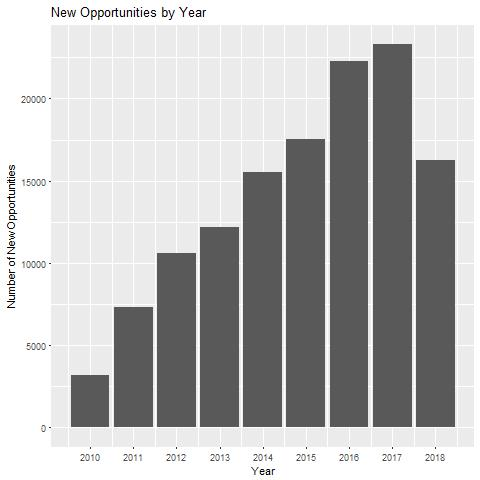
\includegraphics[width=0.9\textwidth]{formsByYear_plot.jpg} % first figure itself
        \caption{New Submittable Opportunities by Year}
	  \label{fig:formYear}
    \end{minipage}\hfill
    \begin{minipage}{0.45\textwidth}
        \centering
        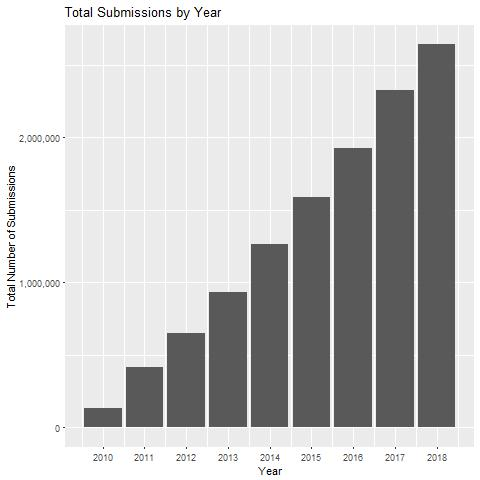
\includegraphics[width=0.9\textwidth]{subsByYear_plot.jpg} % second figure itself
        \caption{Total Number of Submissions Made by Year}
	  \label{fig:subYear}
    \end{minipage}
\end{figure}
\FloatBarrier
On average, opportunities which have received at least one submission have received 125 submissions, with a range from one to 145K. About 75\% of opportunities have received at least one submission, 45\% have received at least five submissions, and 30\% have received over 20 submissions. The intermittent nature of many opportunities makes it difficult to define what should be considered an ``active" opportunity, but Figure \ref{fig:activeForms} shows the number of opportunities that received at least one submission each year. These numbers follow a similar, though less dramatic, pattern as the number of new opportunities each year (Figure \ref{fig:formYear}), steadily increasing until 2018.

Each opportunity has various textual data associated with it, including the opportunity name, a brief description of the opportunity, and any number of form field descriptions. A formfield description can be anything that the organization wants to put on their online form, from something as simple as ``Name:" to a full writing prompt or detailed submission instructions. The opportunity descriptions also vary greatly in their descriptive usefulness, some consisting of multiple paragraphs describing the opportunity guidelines in detail, and others simply stating ``Complete the form below". 

\begin{figure}[h]
    \centering
    \begin{minipage}{0.45\textwidth}
        \centering
        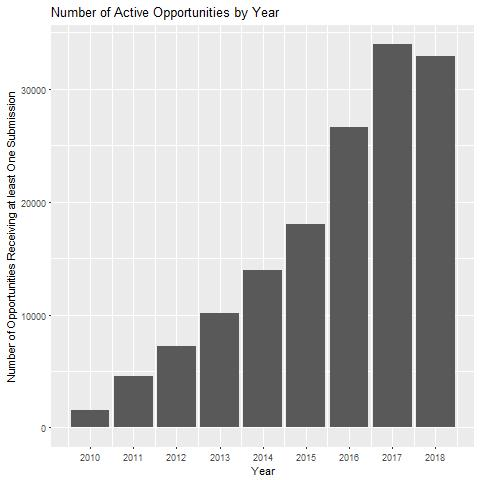
\includegraphics[width=0.9\textwidth]{activeForms_plot.jpg} % first figure itself
        \caption{Number of Opportunities Receiving at least One Submission by Year}
	  \label{fig:activeForms}
    \end{minipage}\hfill
\end{figure}
\FloatBarrier

\section{Labels}
As Submittable has grown, it has seen several generations of labeling methodologies. Currently, the only actively-updated labels are ``usecase" labels applied at the organizational level, and ``discover" labels applied at the opportunity level. The usecase labels are assigned by account managers and are meant to describe what type of opportunities the organization will offer, such as ``publishing", ``fellowships", or ``grants". The discover labels are assigned by the organizations themselves as they opt in to Submittable's opportunity search engine (called ``Discover"), and can be anything from a list of almost 200 options that they think submitters might search for in relation to their opportunity. The full lists of usecase and discover labels can be found in Appendix \ref{app:labels}

Only about 40K opportunities are associated with a usecase label (ie. are hosted by an organization with a usecase label), but this makes sense since the labels only started being applied in a consistent manner in the last year, and there were roughly 40K active opportunities in 2018. The ten usecase labels with the highest number of associated opportunities are shown in Table \ref{table:topusecase}.  

67K discover labels are associated with opportunities, however, since the relationship between the discover label and an opportunity is many-to-one, only 20K unique opportunities are associated with discover labels. Also, since many of the discover labels are overlapping (ie. ``book" vs. ``memoir" vs. ``stories"), I needed to map these onto broader category labels. Submittable identified grant applicants, filmmakers, photographers, and writers (with the subcategories of poetry, fiction, and non-fiction writers), so I grouped the discover labels under these categories. Table \ref{table:discovergroup} shows the number of unique forms with discover labels that fall into these categories. Since we know that only 20K unique opportunities are associated with discover labels, this table (which sums to about 40K) reiterates the many-to-one relationship between discover labels and opportunities.
\begin{figure}[h]
\begin{minipage}{0.45\textwidth}
\centering
\captionof{table}{Top Ten Usecase Labels}
\label{table:topusecase}
\begin{tabular}{rlr}
  \hline
 & Usecase & Count \\ 
  \hline
1 & Publishing & 10836 \\ 
  2 & Grants & 7406 \\ 
  3 & Contest & 4938 \\ 
  4 & Award/ Nomination & 4283 \\ 
  5 & Exhibition & 2626 \\ 
  6 & Conference & 2342 \\ 
  7 & Festival or Event & 1879 \\ 
  8 & Other & 1631 \\ 
  9 & Fellowship & 1613 \\ 
  10 & Scholarships & 1311 \\ 
   \hline
\end{tabular}
\end{minipage}
\hfill
\begin{minipage}{0.45\textwidth}
     \centering
\captionof{table}{Grouped Discover Labels}
\label{table:discovergroup}
\centering
\begin{tabular}{rlr}
  \hline
 & Discover Group & Count \\ 
  \hline
1 & Fiction & 9871 \\ 
  2 & Film & 5302 \\ 
  3 & Grant & 3157 \\ 
  4 & Nonfiction & 8311 \\ 
  5 & Photography & 5451 \\ 
  6 & Poetry & 8100 \\ 
   \hline
\end{tabular}
    \end{minipage}
\end{figure}
\FloatBarrier


\chapter{Methodology}

\section{Data Selection}

- only interested in submitters who have submitted more than once in the last two years

- will include both opted-in and not in the ranking to capture more "un-labeled" submitters and strengthen the network effects; then filter post-hoc to meet data privacy standards? Check with Bruce

- limit to opportunities from last two years as well? May be necessary for size restrictions d/t text data

\section{Topic-weighted ranking vector}

- keyword lists: filmmaker, photographer, writer (fiction, poetry, nonfiction), grants

- weighting for labels vs. keyword use in product descriptions vs. keyword use in user descriptions

--- 1 pt for ea submission to opportunity w/ keyword match (for each keyword?); 2 pt for label match; 2 pt for user keyword match (for each keyword, added for multiple matches of same keyword?)

--- should opportunities be penalized if they have multiple labels/keywords from different keyword lists?

- every user gets 1 to start out with? so that they aren't precluded from results d/t failure to keyword match? allows for connection only via common submissions w/ other highly topical submitters

\section{PageRank Adaptation}

-Basic PageRank algorithm function

- Discussion of how topic-weighted vector applied

\section{How to Measure Success}

- compare results to keyword match lists

- if time: compare response rate (click-through or even email open) for pagerank-developed list vs. keyword match

- discussion of cost balance for bigger vs. more targeted list for marketing purposes; ranked vector may be good, allow for multiple email campaigns or fudging of lists as needed?

\chapter{Results}
\chapter{Conclusion}        

\appendix
\appendixpage
\addappheadtotoc
\section{Label Lists}
\label{app:labels}
\begin{minipage}{0.5\textwidth}
\centering
\begin{tabular}{rl}
  \hline
 & Usecase \\ 
  \hline
1 & Publishing \\ 
  2 & Other \\ 
  3 & Admissions \\ 
  4 & Scholarships \\ 
  5 & Job applications \\ 
  6 & Fellowship \\ 
  7 & Festival or Event \\ 
  8 & Peer Review \\ 
  9 & Artwork submissions \\ 
  10 & Audition \\ 
  11 & Grant applications \\ 
  12 & Contest or Campaign Entries \\ 
  13 & Video/Audio submissions \\ 
  14 & Award/ Nomination \\ 
  15 & Contest \\ 
  16 & Grants \\ 
  17 & Conference \\ 
  18 & Exhibition \\ 
  19 & Residency \\ 
  20 & Manuscript/Content submissions \\ 
  21 & Internal Use \\ 
  22 & Fellowship applications \\ 
  23 & Internships \\ 
  24 & Festival or Event submissions \\ 
  25 & Corporate Giving \\ 
  26 & Conference submissions \\ 
  27 & General applications \\ 
  28 & Audition submissions \\ 
   \hline
\end{tabular}
\end{minipage}
\newpage


\begin{minipage}{0.24\textwidth}

\begin{tabular}{rl}
  \hline
 & Discover.Label \\ 
  \hline
1 & interviews \\ 
  2 & book \\ 
  3 & review \\ 
  4 & art \\ 
  5 & fiction \\ 
  6 & prose \\ 
  7 & literary \\ 
  8 & short-story \\ 
  9 & video \\ 
  10 & submishmash \\ 
  11 & nonfiction \\ 
  12 & memoir \\ 
  13 & essay \\ 
  14 & stories \\ 
  15 & travel \\ 
  16 & visual-art \\ 
  17 & creative-writing \\ 
  18 & scripts \\ 
  19 & contest \\ 
  20 & theme \\ 
  21 & publishing \\ 
  22 & manuscript \\ 
  23 & science-fiction \\ 
  24 & drawing \\ 
  25 & painting \\ 
  26 & photography \\ 
  27 & nonprofit \\ 
  28 & chapbook \\ 
  29 & lyrics \\ 
  30 & critique \\ 
  31 & sculpture \\ 
  32 & classes \\ 
  33 & experimental \\ 
  34 & blog \\ 
  35 & for-sale \\ 
  36 & monologue \\ 
  37 & design \\ 
  38 & sports \\ 
  39 & podcast \\ 
  40 & academic \\ 
  41 & television \\ 
  42 & sound \\ 
  43 & collaborative \\ 
  44 & international \\ 
  45 & graphic-novel \\ 
  46 & article \\ 
  47 & short-play \\ 
  48 & theater \\ 
  49 & erotica \\ 
  50 & job \\ 
  \hline
\end{tabular}
    \end{minipage}
\begin{minipage}{0.24\textwidth}

\begin{tabular}{rl}
  \hline
 & Discover.Label \\ 
  \hline
  51 & science \\ 
  52 & criticism \\ 
  53 & hybrid \\ 
  54 & dance \\ 
  55 & student \\ 
  56 & exhibition \\ 
  57 & philosophy \\ 
  58 & military \\ 
  59 & grant \\ 
  60 & native-american \\ 
  61 & children \\ 
  62 & column \\ 
  63 & health \\ 
  64 & politics \\ 
  65 & culture \\ 
  66 & social-justice \\ 
  67 & volunteer \\ 
  68 & animation \\ 
  69 & speculative \\ 
  70 & subscribe \\ 
  71 & print \\ 
  72 & festival \\ 
  73 & multilingual \\ 
  74 & comedy \\ 
  75 & humor \\ 
  76 & conference \\ 
  77 & retreat \\ 
  78 & environmental \\ 
  79 & scholarships \\ 
  80 & public-art \\ 
  81 & cover-art \\ 
  82 & independent \\ 
  83 & workspace \\ 
  84 & art-fair \\ 
  85 & african-american \\ 
  86 & paranormal \\ 
  87 & juried \\ 
  88 & season \\ 
  89 & asian-american \\ 
  90 & alcohol \\ 
  91 & fashion \\ 
  92 & midwest \\ 
  93 & VR/360 \\ 
  94 & female \\ 
  95 & VR \\ 
  96 & public-media \\ 
  97 & civil-rights \\ 
  98 & mental-health \\ 
  99 & journal \\ 
  100 & poetry \\ 
  \hline
\end{tabular}
    \end{minipage}
\begin{minipage}{0.24\textwidth}

\begin{tabular}{rl}
  \hline
 & Discover.Label \\ 
  \hline
  101 & magazine \\ 
  102 & anthology \\ 
  103 & writing \\ 
  104 & flash \\ 
  105 & feedback \\ 
  106 & short-film \\ 
  107 & screenwriting \\ 
  108 & feminist \\ 
  109 & young-adult \\ 
  110 & novel \\ 
  111 & agent \\ 
  112 & online \\ 
  113 & magical-realism \\ 
  114 & translation \\ 
  115 & adventure \\ 
  116 & award \\ 
  117 & residency \\ 
  118 & plays \\ 
  119 & haiku \\ 
  120 & community \\ 
  121 & business \\ 
  122 & funding \\ 
  123 & editor \\ 
  124 & digital \\ 
  125 & book-arts \\ 
  126 & journalism \\ 
  127 & audio \\ 
  128 & surrealist \\ 
  129 & documentary \\ 
  130 & film \\ 
  131 & mystery \\ 
  132 & technology \\ 
  133 & comics \\ 
  134 & pitch \\ 
  135 & illustration \\ 
  136 & religion \\ 
  137 & fellowship \\ 
  138 & performance \\ 
  139 & prize \\ 
  140 & romance \\ 
  141 & horror \\ 
  142 & education \\ 
  143 & lgbtqia \\ 
  144 & fantasy \\ 
  145 & food \\ 
  146 & architecture \\ 
  147 & spoken-word \\ 
  148 & indigenous \\ 
  149 & readings \\ 
  150 & media \\ 
 \hline
\end{tabular}
    \end{minipage}
\begin{minipage}{0.24\textwidth}

\begin{tabular}{rl}
  \hline
 & Discover.Label \\ 
  \hline
  151 & music \\ 
  152 & canada \\ 
  153 & gallery \\ 
  154 & mythology \\ 
  155 & emerging \\ 
  156 & event \\ 
  157 & music-composition \\ 
  158 & parenting \\ 
  159 & minorities \\ 
  160 & crafts \\ 
  161 & printmaking \\ 
  162 & workshop \\ 
  163 & internship \\ 
  164 & novella \\ 
  165 & mentorship \\ 
  166 & history \\ 
  167 & ceramics \\ 
  168 & museum \\ 
  169 & orchestra \\ 
  170 & new-york \\ 
  171 & fiber-arts \\ 
  172 & paper \\ 
  173 & poster \\ 
  174 & thriller \\ 
  175 & 360-Video \\ 
  176 & tequila \\ 
  177 & service-learning \\ 
   \hline
\end{tabular}

    \end{minipage}

\begin{thebibliography}{9}
  % type bibliography here
\end{thebibliography}

\end{document}